% This LaTeX was auto-generated from MATLAB code.
% To make changes, update the MATLAB code and export to LaTeX again.

\documentclass{article}

\usepackage[utf8]{inputenc}
\usepackage[T1]{fontenc}
\usepackage{lmodern}
\usepackage{graphicx}
\usepackage{color}
\usepackage{hyperref}
\usepackage{amsmath}
\usepackage{amsfonts}
\usepackage{epstopdf}
\usepackage[table]{xcolor}
\usepackage{matlab}
\usepackage{geometry}

\sloppy
\epstopdfsetup{outdir=./}
\graphicspath{ {./main_images/} }

\geometry{left=1.0in,right=1.0in,top=1.0in,bottom=1.0in}

\begin{document}

\title{Homework 1 Report}
\author{Zhikun Lu\footnote{Economics Department, Emory University. I collaborate with Tianhao Zhao and Xiang Cheng in this project. They generously shared their code with me and provided insightful discussions.}}
\date{\today}
\maketitle

% \matlabtitle{Homework 1 Report}

We use Dynare 4.6.2 for this homework. Dynare 4.6 has changed the usage of some functions, for example, \textit{stoch\_simul}, and thus the code may not work for a lower version.

\begin{matlabcode}
addpath('/Applications/Dynare/4.6.2/matlab'); % add dynare path
\end{matlabcode}

\section*{Exercise 4.10} 

Before starting Q1, we first replicate the right panel of table 4.2 in the textbook to ensure our model, variable definitions, and solution method are consistent with the textbook.

\begin{matlabcode}
dynare Q410.mod; 
print_table()    % exactly replicate table 4.2 using textbook calibration
\end{matlabcode}
\begin{matlaboutput}
Results of table 4.2:

Variable  sig_x       rho1       rho2
   y       3.08       0.62       1.00
   c       2.71       0.78       0.84
   i       9.04       0.07       0.67
   h       2.12       0.62       1.00
tb_y       1.78       0.51      -0.04
ca_y       1.45       0.32       0.05
\end{matlaboutput}

\subsection*{Q1. Calibrate the EDEIR Model for Canada 1960-2011}

\begin{matlabcode}
%{
NOTE:
    1. moments to match: [std(y),autocor(y),std(i),std(tb/y)]
    2. target moment values: [3.71%, 0.86, 10.31%, 1.72%]
    3. pars to calibrate: rho, eta, phi, psi_1
    4. method: min distance
    5. solver: fminunc/BFGS Quasi-Newton
    6. init guess: param = [0.42 0.0129 0.028 0.000742]
%}

param_init = [0.42 0.0129 0.028 0.000742];
param_est  = fminunc(@(x)m_dist(x), param_init);

fprintf('Estimation results:\n');
fprintf('\n');
fprintf('rho   = %.6f\n', param_est(1));
fprintf('eta   = %.6f\n', param_est(2));
fprintf('phi   = %.6f\n', param_est(3));
fprintf('psi_1 = %.6f\n', param_est(4));
\end{matlabcode}

\begin{matlaboutput}
Estimation results:

rho   = 0.621901
eta   = 0.010536
phi   = 0.018179
psi_1 = 0.026189
\end{matlaboutput}

Thus, we get a higher $\rho$ and $\psi_1$ but a lower $\eta$ and $\phi$.



\subsection*{Q2. Compute the Theoretical Second Moments}

We employ the estimated parameters to re-solve the model. Dynare automatically reports the theoretical moments for 1st order solutions.
\begin{matlabcode}
% Q2 Compute theoretical second moments

set_param_value('rho',  param_est(1)); 
set_param_value('eta',  param_est(2));
set_param_value('phi',  param_est(3)); 
set_param_value('psi_1',param_est(4));

[info,oo_,options_,M_] = stoch_simul(M_,options_,oo_,var_list_);

print_table()
\end{matlabcode}

\begin{matlaboutput}
Results of table 4.2:

Variable  sig_x       rho1       rho2
   y       3.71       0.84       1.00
   c       3.18       0.89       0.98
   i      10.31       0.16       0.64
   h       2.55       0.84       1.00
tb_y       1.73       0.04      -0.12
ca_y       1.66       0.04      -0.07
\end{matlaboutput}

\subsection*{Q3. Comment}

\begin{itemize}
    \item The model does a good job in generating the observed standard deviation of output $y$, investment $i$, and trade-balance-to-output ratio $\frac{tb}{y}$.\\
    But this is not surprising because that is how we calibrate the model using the SMM. 
    
    \item The model does a poor job in explaining the autocorrelation of $i$ and $\frac{tb}{y}$, which are much less correlated than in the data.

    \item The model also does a poor job in explaining the correlation between $y$ and $\frac{tb}{y}$. Its sign is the opposite of the one in the data.
\end{itemize}

\subsection*{Q4. TFP Shock and Output Volatility}

\begin{matlabcode}
% Q4 compute std(ln A)
sd_list  = sqrt(diag(oo_.var));
sd_A     = sd_list(strcmp('A',M_.endo_names))*100;
sd_y     = sd_list(strcmp('y',M_.endo_names))*100;
sd_A_old = 100*sqrt(0.0129^2/(1-0.42^2));

fprintf('Unconditional SD(ln(A)) = %.4f\n', sd_A);
fprintf('Old value:                %.4f\n', sd_A_old);

fprintf('Unconditional SD(y)     = %.4f\n', sd_y);
fprintf('Old value:                %.4f\n', 3.08);
\end{matlabcode}

\begin{matlaboutput}
Unconditional SD(ln(A)) = 1.3455
Old value:                1.4214
Unconditional SD(y)     = 3.7130
Old value:                3.0800
\end{matlaboutput}

From the results above we can see that 
\begin{itemize}
    \item the volatility of TFP shock has actually \textbf{decreased}; 
    \item On the other hand, the volatility of output has \textbf{increased}. 
\end{itemize}
This means the business cycle relies less on the TFP shock. However, its internal amplification and propagation mechanisms have become stronger than in the past. The latter effect outweighs the previous effect, and as a result, the overall output volatility still increases.


\clearpage

\section{Exercise 5.2} 

\subsection*{Q1. Equilibrium Conditions}

There are 21 variables: $C_{t}, h_{t}, A_{t}, I_{t}, Z_{t}, X_{t}, D_{t}, R_{t}, g_{t}, \widetilde{D}_{t}, A_{t}^{T}, A_{t}^{N}, Y_{t}^{T}, Y_{t}^{N}, K_{t}^{T}, K_{t}^{N}, h_{t}^{T}, h_{t}^{N}, I_{t}^{T}, I_{t}^{N}, \lambda_{t}$.

Accordingly, there are 21 equations for the equilibrium:
\begin{align}
A_{t}&=C_{t}+I_{t} \\
A_{t}&=\left[\eta\left(A_{t}^{T}\right)^{1- \frac{1}{\mu}}+(1-\eta)\left(A_{t}^{N}\right)^{1- \frac{1}{\mu}}\right]^{1 /(1- \frac{1}{\mu})} \\
Y_{t}^{T}&=Z_{t}\left(K_{t}^{T}\right)^{1-\alpha_{T}}\left(X_{t} h_{t}^{T}\right)^{\alpha_{T}} \\
Y_{t}^{N}&=Z_{t}\left(K_{t}^{N}\right)^{1-\alpha_{N}}\left(X_{t} h_{t}^{N}\right)^{\alpha_{N}} \\
K_{t+1}^{T}&=(1-\delta) K_{t}^{T}+I_{t}^{T}-\frac{\phi}{2}\left(\frac{K_{t+1}^{T}}{K_{t}^{T}}-g\right)^{2} K_{t}^{T} \\
K_{t+1}^{N}&=(1-\delta) K_{t}^{N}+I_{t}^{N}-\frac{\phi}{2}\left(\frac{K_{t+1}^{N}}{K_{t}^{N}}-g\right)^{2} K_{t}^{N} \\
I_{t}&=I_{t}^{T}+I_{t}^{N} \\
Y_{t}^{N}&=A_{t}^{N} \\
h_{t}&=h_{t}^{T}+h_{t}^{N} \\
\frac{D_{t+1}}{R_{t}}&=D_{t}+A_{t}^{T}-Y_{t}^{T}\\
R_{t}&=R^{*}+\psi\left[e^{\widetilde{D}_{t+1} / X_{t}-\bar{d}}-1\right] \\
\widetilde{D}_{t}&=D_{t} \\
\ln Z_{t}&=\rho_{Z} \ln Z_{t-1}+\sigma_{Z} \varepsilon_{t}^{Z} \\
\ln \left(\frac{g_{t}}{g}\right)&=\rho_{g} \ln \left(\frac{g_{t-1}}{g}\right)+\sigma_{g} \varepsilon_{t}^{g} \\
g_{t}&=\frac{X_{t}}{X_{t-1}} \\
\lambda_{t}&=\beta^{t}\left[C_{t}^{\gamma}\left(1-h_{t}\right)^{1-\gamma}\right]^{-\sigma} \left(1-h_{t}\right)^{1-\gamma}  \gamma  C_{t}^{\gamma-1} \\
\beta^{t}\left[C_{t}^{\gamma}\left(1-h_{t}\right)^{1-\gamma}\right]^{-\sigma} \left(1-h_{t}\right)^{-\gamma} (1-\gamma)  C_{t}^{\gamma}&=\lambda_{t} A_t^{\frac{1}{\mu}} \eta\left(A_{t}^{T}\right)^{- \frac{1}{\mu}} \alpha_{T} Z_{t} X_{t}\left(\frac{K_{t}^{T}}{X_{t} h_{t}^{T}}\right)^{1-\alpha_{T}} \\
\beta^{t}\left[C_{t}^{\gamma}\left(1-h_{t}\right)^{1-\gamma}\right]^{-\sigma} \left(1-h_{t}\right)^{-\gamma} (1-\gamma)  C_{t}^{\gamma}&=\lambda_{t} A_t^{\frac{1}{\mu}}(1-\eta)\left(A_{t}^{N}\right)^{- \frac{1}{\mu}} \alpha_{N} Z_{t} X_{t}\left(\frac{K_{t}^{N}}{X_{t} h_{t}^{N}}\right)^{1-\alpha_{N}}\\
\lambda_{t} A_t^{\frac{1}{\mu}} \eta\left(A_{t}^{T}\right)^{-1 / \mu} \frac{1}{R_{t}}&=E_{t} \lambda_{t+1}A_{t+1}^{\frac{1}{\mu}} \eta\left(A_{t+1}^{T}\right)^{-1 / \mu} 
\end{align}
\begin{align}
\lambda_{t}\left(1+\phi\left(\frac{K_{t+1}^{T}}{K_{t}^{T}}-g\right)\right)&=E_{t} \lambda_{t+1}\left\{ A_{t+1}^{\frac{1}{\mu}} \eta\left(A_{t+1}^{T}\right)^{-\frac{1}{\mu}}\left(1-\alpha_{T}\right) \frac{Y_{t+1}^{T}}{K_{t+1}^{T}}+1-\delta+\phi\left(\frac{K_{t+2}^{T}}{K_{t+1}^{T}}-g\right) \frac{K_{t+2}^{T}}{K_{t+1}^{T}}-\frac{\phi}{2}\left(\frac{K_{t+2}^{T}}{K_{t+1}^{T}}-g\right)^{2}\right\} \\
\lambda_{t}\left(1+\phi\left(\frac{K_{t+1}^{N}}{K_{t}^{N}}-g\right)\right)&=E_{t} \lambda_{t+1}\left\{A_{t+1}^{\frac{1}{\mu}}(1-\eta)\left(A_{t+1}^{N}\right)^{-\frac{1}{\mu}}\left(1-\alpha_{N}\right) \frac{Y_{t+1}^{N}}{K_{t+1}^{N}}+1-\delta+\phi\left(\frac{K_{t+2}^{N}}{K_{t+1}^{N}}-g\right) \frac{K_{t+2}^{N}}{K_{t+1}^{N}}-\frac{\phi}{2}\left(\frac{K_{t+2}^{N}}{K_{t+1}^{N}}-g\right)^{2}\right\}
\end{align}

\subsection*{Q2. Prices}
From the FOCs, it is easy to derive
\begin{align*}
p_{t}^{N}&=\frac{1-\eta}{\eta}\left(\frac{A_{t}^{N}}{A_{t}^{T}}\right)^{-\frac{1}{\mu}},\\
p_{t}&=\left[\eta\left(A_{t}^{T}\right)^{1-\frac{1}{\mu}}+(1-\eta)\left(A_{t}^{N}\right)^{1-\frac{1}{\mu}}\right]^{\frac{1}{1-\mu}} \eta^{-1}\left(A_{t}^{T}\right)^{1 / \mu}.
\end{align*}
Both of them are stationary variables. This is because their values only depend on the ratio, $\frac{A_{t}^{N}}{A_{t}^{T}}$, which is a constant along the BGP.

\subsection*{Q3. Stationary Form of the Equilibrium Conditions}

Define stationary variables as follows:
\begin{align*}
&
\hat{c}_{t} \equiv \frac{C_{t}}{X_{t-1}}, 
\hat{a}_{t} \equiv \frac{A_{t}}{X_{t-1}}, 
\hat{\imath}_{t} \equiv \frac{I_{t}}{X_{t-1}}, 
\hat{d}_{t} \equiv \frac{D_{t}}{X_{t-1}}, 
\hat{r}_{t} \equiv \frac{R_{t}}{X_{t-1}}, 
\hat{a}_{t}^{T} \equiv \frac{A_{t}^{T}}{X_{t-1}}, 
\hat{a}_{t}^{N} \equiv \frac{A_{t}^{N}}{X_{t-1}}, 
\widehat{y}_{t}^{T} \equiv \frac{Y_{t}^{T}}{X_{t-1}},\\
&\hat{y}_{t}^{N} \equiv \frac{Y_{t}^{N}}{X_{t-1}}, 
\hat{k}_{t}^{T} \equiv \frac{K_{t}^{T}}{X_{t-1}}, 
\hat{k}_{t}^{N} \equiv \frac{K_{t}^{N}}{X_{t-1}}, 
\hat{\imath}_{t}^{T} \equiv \frac{I_{t}^{T}}{X_{t-1}}, 
\hat{l}_{t}^{N} \equiv \frac{I_{t}^{N}}{X_{t-1}}, 
\hat{\lambda}_{t} \equiv X_{t-1}^{1+(\sigma-1)\gamma}\lambda_{t}.
\end{align*}
Then, the stationary form equilibrium conditions can be written as follows:
\begin{align}
\hat{a}_{t}&=\hat{c}_{t}+\hat{\imath}_{t} \\
\hat{a}_{t}&=\left[\eta\left(\hat{a}_{t}^{T}\right)^{1-1 / \mu}+(1-\eta)\left(\hat{a}_{t}^{N}\right)^{1-1 / \mu}\right]^{1 /(1-1 / \mu)} \\
\hat{y}_{t}^{T}&=Z_{t}\left(\hat{k}_{t}^{T}\right)^{1-\alpha_{T}}\left(g_{t} h_{t}^{T}\right)^{\alpha_{T}} \\
\hat{y}_{t}^{N}&=Z_{t}\left(\hat{k}_{t}^{N}\right)^{1-\alpha_{N}}\left(g_{t} h_{t}^{N}\right)^{\alpha_{N}} \\
\hat{k}_{t+1}^{T}&=\frac{(1-\delta) \hat{k}_{t}^{T}+\hat{\imath}_{t}^{T}-\frac{\phi}{2}\left(\frac{\hat{k}_{t+1}^{T}}{\hat{k}_{t}^{T}} g_{t}-g\right)^{2} \hat{k}_{t}^{T}}{g_{t}} \\
\hat{k}_{t+1}^{N}&=\frac{(1-\delta) \hat{k}_{t}^{N}+\hat{\imath}_{t}^{N}-\frac{\phi}{2}\left(\frac{\hat{k}_{t+1}^{N}}{\hat{k}_{t}^{N}} g_{t}-g\right)^{2} \hat{k}_{t}^{N}}{g_{t}} \\
\hat{\imath}_{t}&=\hat{\imath}_{t}^{T}+\hat{\imath}_{t}^{N} \\
\hat{y}_{t}^{N}&=\hat{a}_{t}^{N} \\
h_{t}&=h_{t}^{T}+h_{t}^{N} \\
\frac{\hat{d}_{t+1} g_{t}}{R_{t}}&=\hat{d}_{t}+\hat{a}_{t}^{T}-\hat{y}_{t}^{T}\\
R_{t}&=R^{*}+\psi\left[e^{\hat{d}_{t+1}-\bar{d}}-1\right] \\
\ln Z_{t}&=\rho_{Z} \ln Z_{t-1}+\sigma_{Z} \varepsilon_{t}^{Z} \\
\ln \left(g_{t} / g\right)&=\rho_{g} \ln \left(g_{t-1} / g\right)+\sigma_{g} \varepsilon_{t}^{g} \\
g_{t}&=\frac{X_{t}}{X_{t-1}}
\end{align}
\begin{align}
(1-\gamma) \hat{c}_{t}&=\gamma\left(1-h_{t}\right)\hat{a}_{t}^{1/\mu} \eta\left(\hat{a}_{t}^{T}\right)^{-1 / \mu} \alpha_{T} Z_{t} g_{t}\left(\frac{\hat{k}_{t}^{T}}{g_{t} n_{t}^{T}}\right)^{1-\alpha_{T}} \\
(1-\gamma) \hat{c}_{t}&=\gamma\left(1-h_{t}\right)\hat{a}_{t}^{1/\mu}(1-\eta)\left(\hat{a}_{t}^{N}\right)^{-1 / \mu} \alpha_{N} Z_{t} g_{t}\left(\frac{\hat{k}_{t}^{N}}{g_{t} h_{t}^{N}}\right)^{1-\alpha_{N}}
\end{align}
\begin{align}
\left(1-h_{t}\right)^{(1-\gamma)(1-\sigma)}  \gamma  \hat{c}_{t}^{\gamma-1-\sigma\gamma} \hat{a}_{t}^{1/\mu} \eta\left(\hat{a}_{t}^{T}\right)^{-1 / \mu} = E_{t} \beta R_{t} g_{t}^{-\sigma \gamma}\left(1-h_{t+1}\right)^{(1-\gamma)(1-\sigma)}  \gamma  \hat{c}_{t+1}^{\gamma-1-\sigma\gamma} g_{t}^{\gamma-1} \hat{a}_{t+1}^{1/\mu} \eta\left(\hat{a}_{t+1}^{T}\right)^{-1 / \mu}
\end{align}
\begin{align}
\begin{aligned}
&\left[\hat{c}_{t}^{\gamma}\left(1-h_{t}\right)^{1-\gamma}\right]^{-\sigma} \left(1-h_{t}\right)^{1-\gamma} \gamma \hat{c}_{t}^{\gamma-1}\left(1+\phi\left(\frac{\hat{k}_{t+1}^{T}}{\hat{k}_{t}^{T}} g_{t}-g\right)\right)=E_{t} \beta\left[\hat{c}_{t+1}^{\gamma} g_{t}^{\gamma}\left(1-h_{t+1}\right)^{1-\gamma}\right]^{-\sigma} \left(1-h_{t+1}\right)^{1-\gamma} \gamma \hat{c}_{t+1}^{\gamma-1} g_{t}^{\gamma-1}\\
&\quad \quad \left\{\eta\left(\frac{\hat{a}_{t+1}}{\hat{a}_{t+1}^{T}}\right)^{\frac{1}{\mu}}\left(1-\alpha_{T}\right) \frac{\hat{a}_{t+1}^{T}}{\hat{k}_{t+1}^{T}}+1-\delta+\phi\left(\frac{\hat{k}_{t+2}^{T}}{\hat{k}_{t+1}^{T}} g_{t+1}-g\right) \frac{\hat{k}_{t+2}^{T}}{\hat{k}_{t+1}^{T}} g_{t+1}-\frac{\phi}{2}\left(\frac{\hat{k}_{t+2}^{T}}{\hat{k}_{t+1}^{T}} g_{t+1}-g\right)^{2}\right\}
\end{aligned}
\end{align}
\begin{align}
\begin{aligned}
&\left[\hat{c}_{t}^{\gamma}\left(1-h_{t}\right)^{1-\gamma}\right]^{-\sigma} \left(1-h_{t}\right)^{1-\gamma} \gamma \hat{c}_{t}^{\gamma-1}\left(1+\phi\left(\frac{\hat{k}_{t+1}^{N}}{\hat{k}_{t}^{N}} g_{t}-g\right)\right)=E_{t} \beta\left[\hat{c}_{t+1}^{\gamma} g_{t}^{\gamma}\left(1-h_{t+1}\right)^{1-\gamma}\right]^{-\sigma} \left(1-h_{t+1}\right)^{1-\gamma} \gamma \hat{c}_{t+1}^{\gamma-1} g_{t}^{\gamma-1}\\
&\quad \quad \left\{(1-\eta)\left(\frac{\hat{a}_{t+1}}{\hat{a}_{t+1}^{N}}\right)^{\frac{1}{\mu}}\left(1-\alpha_{N}\right) \frac{\hat{a}_{t+1}^{N}}{\hat{k}_{t+1}^{N}}+1-\delta+\phi\left(\frac{\hat{k}_{t+2}^{T}}{\hat{k}_{t+1}^{N}} g_{t+1}-g\right) \frac{\hat{k}_{t+2}^{T}}{\hat{k}_{t+1}^{N}} g_{t+1}-\frac{\phi}{2}\left(\frac{\hat{k}_{t+2}^{N}}{\hat{k}_{t+1}^{N}} g_{t+1}-g\right)^{2}\right\}
\end{aligned}
\end{align}

\subsection*{Q4. Steady State}

\begin{matlabcode}
% calibrate the model and saves the steady state
param.beta       = 0.98;
param.gamma      = 0.36;
param.d_bar      = 0.10;
param.psi        = 0.001;
param.alpha_T    = 0.40;
param.alpha_N    = 0.80;
param.delta      = 0.05;
param.g_bar      = 1.0066;
param.phi        = 1.37;
param.miu        = 0.44;
param.sigma      = 2;
% share paremeter of tradable goods; to be calibrated endogenously
param.yeta       = 0.5; 
% solve for the steady state with eta = 0.5, an initial guess
% x_ss0 provides an initial guess for the steady state
x0    = [0,0,0.1,1,1,1,1,1,1,1,1,1,1,1,1,1];
x_ss0 = fsolve(@(x)ss_model(x,param), x0);
% find the eta
eeta = fsolve(@(x)calibrate_eta(x,param,x_ss0), param.yeta);
% update the parameters and the steady state vals
[~, param, x_ss] = calibrate_eta(eeta, param, x_ss0);
\end{matlabcode}

We find $\eta =  0.349.$ Passing this $\eta$ into Dynare, the steady state is reported in Dynare as follows:

\begin{matlabcode}
dynare Ex502.mod
\end{matlabcode}

\begin{matlaboutput}
STEADY-STATE RESULTS:

c            0.224174
h            0.32947
a            0.295923
i            0.0717491
d            0.1
r            1.02958
a_T          0.296406
a_N          0.295665
y_T          0.298638
y_N          0.295665
k_T          0.78296
k_N          0.484693
i_T          0.0443155
i_N          0.0274336
h_T          0.0698872
h_N          0.259583
lambda       3.55303
z            1
g            1.0066
p            2.87583
p_N          1.87583
tb           0.00077606
\end{matlaboutput}

\subsection*{Q5. The Law of Motion}

Dynare also reports the transition function for all variables. The following output has been trimmed. Note that the model is solved without taking logs.

\begin{matlaboutput}
POLICY AND TRANSITION FUNCTIONS
                     z              d            k_T             k_N        
Constant      1.000000       0.100000       0.782960        0.484693        
z(-1)         0.950000       0.207817       0.193557        0.111752        
d(-1)                0       1.020164       0.010874        0.000190        
k_T(-1)              0      -0.390975       0.886212       -0.011684        
k_N(-1)              0       0.072941       0.130435        0.847934        
ez            0.005300       0.001159       0.001080        0.000623        
eg                   0       0.003594      -0.016149       -0.008560        
\end{matlaboutput}

Thus, for a state vector $[z, d, k^{T}, k^{N}]'$, we have
\begin{align*}
h_{x} = \begin{bmatrix}
   0.95 &      0 &     0 &     0\\
   0.20 &   1.02 & -0.39 &  0.07\\
   0.19 &   0.01 &  0.88 &  0.13\\
   0.11 &   0.00 & -0.01 &  0.84\\
\end{bmatrix},
\end{align*}
and its eigenvalues are 
\begin{align*}
\begin{bmatrix}
    0.8883 + 0.0155i &
    0.8883 - 0.0155i &
    0.9776 &
    0.9500 
\end{bmatrix},
\end{align*}
all of which falls within the unit circle. So the system is stable.

\subsection*{Q6. Statitics}

Since $\Delta Y_{t}$, $\Delta C_{t}$, and $tby_{t}$ are all themselves stationary, Dynare can directly report their moments and correlations by carefully defining them in the mod file:

\begin{matlaboutput}
THEORETICAL MOMENTS
VARIABLE     STD. DEV. 
delta_c        0.0173 
delta_y        0.0159 

MATRIX OF CORRELATIONS
Variables     delta_y
delta_c        0.9581
delta_y        1.0000
tby           -0.3035
\end{matlaboutput}

\subsection*{Q7. Moments}

For moments of other non-stationary variables, Dynare does not report them directly. I follow the procedure describe in the textbook to calculate them.

\begin{matlabcode}
% retrieve the simulated sequence
y_tilde = data(strcmp('logY',M_.endo_names),:)
c_tilde = data(strcmp('logC',M_.endo_names),:)
i_tilde = data(strcmp('logI',M_.endo_names),:)
g       = data(strcmp('g'   ,M_.endo_names),:)

% add the trend back
logX = cumsum(log(g))
logC = c_tilde(2:end) + logX(1:end-1)
logY = y_tilde(2:end) + logX(1:end-1)
logI = i_tilde(2:end) + logX(1:end-1)

% use hpfilter to detrend
[~,c] = hpfilter(logC,1600)
[~,y] = hpfilter(logY,1600)
[~,i] = hpfilter(logI,1600)

burnin=1000;
c = c((burnin+1):end)
y = y((burnin+1):end)
i = i((burnin+1):end)
tby = tby((burnin+1):end)
\end{matlabcode}

\begin{matlabcode}
% report selected moments in table 5.2
std(y)*100
std(c)/std(y)
std(i)/std(y)

corr(y(2:end),y(1:end-1))
corr(y,c)
corr(y,i)
\end{matlabcode}

\begin{matlaboutput}
2.1253
1.0677
2.6207
0.7535
0.9519
0.9625
\end{matlaboutput}

\subsection*{Q8. One Sector Model}

Let the tradable sector's share parameter $\eta \to 1$. Then the nontradable sector will become negligible, and the model will be same as the one in Section 5.2.

Since direct setting $\eta = 1$ will cause some numerical issues in Dynare, we instead remove all model equations relate to the nontradable sector. This yields the same model equations as the model in Sector 5.2.

Thus, what we do below is essentially replicate the results of Table 5.2.

\begin{table}[hb]
    \centering
    \begin{tabular}{rrrr}
    \hline
                     & std($\Delta C_{t}$) & std($\Delta Y_{t}$) & corr($\Delta Y_{t}$, $tby_{t}$)  \\ \hline
    One Sector Model & 1.78                & 1.42                & -0.58       \\ 
    Two Sector Model & 1.73                & 1.59                & -0.30       \\ 
    \end{tabular}
\end{table}

\begin{table}[hb]
    \centering
    \begin{tabular}{lrrrr}
    \hline
    Statistics            & Data & Origin Model & One Sector & Two Sector  \\ \hline
    $\sigma(y)$           & 2.40 & 2.13         & 2.16       & 2.12         \\ 
    $\sigma(c)/\sigma(y)$ & 1.26 & 1.10         & 1.08       & 1.06         \\ 
    $\sigma(i)/\sigma(y)$ & 4.15 & 3.83         & 3.91       & 2.62         \\ 
    $\rho(y)$             & 0.83 & 0.82         & 0.82       & 0.75         \\ 
    $\rho(y,c)$           & 0.82 & 0.91         & 0.92       & 0.95         \\ 
    $\rho(y,i)$           & 0.91 & 0.80         & 0.78       & 0.96         \\ \hline
    \end{tabular}
\end{table}

Comparing the 3rd column and the 4th column, we can see that our procedure generates almost the same results.

\subsection*{Q9. Comments}

The most obvious differences we can find from the above table are
\begin{itemize}
  \item $\sigma(i)/\sigma(y)$ is much lower in the two sector model;
  \item corr($\Delta Y_{t}$, $tby_{t}$) is much higher in the two sector model.
\end{itemize}

Here is my explanation:
\begin{itemize}
  \item When the GDP growth rate is high, the economy usually needs more investment. 
  \item For an open economy, it will borrow from the international market. This is why corr($\Delta Y_{t}$, $tby_{t}$) is negative.
  \item The introduction of nontradable sector makes it harder for the economy to pay back its debt, since part of the output is nontradable.
  \item Thus, the economy has less incentive to borrow from the international market to finance investment.
  \item This logic leads to the two main differences listed above. 
\end{itemize}




\clearpage

\section*{Exercise 6.5}
\subsection*{Q1. The EDEIR Model}
\begin{matlabcode}
%---------------- EDEIR ------------------
% replicate column 4 of table 4.4
% make sure the results generated by the new model is consistent with the old results

dynare EDEIR
\end{matlabcode}
\begin{matlaboutput}
THEORETICAL MOMENTS
VARIABLE         MEAN  STD. DEV.   VARIANCE
y              0.3964     0.0308     0.0010
c              0.1106     0.0271     0.0007
i             -1.0795     0.0904     0.0082
h              0.0074     0.0212     0.0004
tb_y           0.0200     0.0178     0.0003
ca_y           0.0000     0.0145     0.0002

MATRIX OF CORRELATIONS
Variables         y       c       i       h    tb_y    ca_y
y            1.0000  0.8440  0.6688  1.0000 -0.0435  0.0503
c            0.8440  1.0000  0.5177  0.8440 -0.3114  0.0654
i            0.6688  0.5177  1.0000  0.6688 -0.6178 -0.7068
h            1.0000  0.8440  0.6688  1.0000 -0.0435  0.0503
tb_y        -0.0435 -0.3114 -0.6178 -0.0435  1.0000  0.8318
ca_y         0.0503  0.0654 -0.7068  0.0503  0.8318  1.0000

COEFFICIENTS OF AUTOCORRELATION
Order          1       2       3       4       5
y         0.6170  0.3603  0.2066  0.1201  0.0733
c         0.7822  0.6367  0.5493  0.4996  0.4721
i         0.0686 -0.1379 -0.1363 -0.0935 -0.0553
h         0.6170  0.3603  0.2066  0.1201  0.0733
tb_y      0.5086  0.3484  0.3028  0.2938  0.2945
ca_y      0.3220  0.0875  0.0130 -0.0067 -0.0096
Total computing time : 0h00m01s
\end{matlaboutput}

We can see that the moments reported in Dynare are basically the same as in table 4.4.

Now we turn off the TFP shock and turn on the interest rate shock.

\begin{matlabcode}
% turn off productivity shock and turn on interest rate shock
set_param_value('eta', 0);
set_param_value('sigma_mu', 0.012);
% re-run the model
options_.irf = 20;
[info,oo_,options_,M_]=stoch_simul(M_,options_,oo_,var_list_);
\end{matlabcode}
\begin{matlaboutput}
THEORETICAL MOMENTS
VARIABLE         MEAN  STD. DEV.   VARIANCE
y              0.3964     0.1560     0.0243
c              0.1106     0.1092     0.0119
i             -1.0795     0.9933     0.9866
h              0.0074     0.1072     0.0115
tb_y           0.0200     0.2417     0.0584
ca_y           0.0000     0.2377     0.0565

MATRIX OF CORRELATIONS
Variables         y       c       i       h    tb_y    ca_y
y            1.0000  0.9932  0.0635  1.0000  0.2357  0.1869
c            0.9932  1.0000  0.1636  0.9932  0.1351  0.0867
i            0.0635  0.1636  1.0000  0.0635 -0.9547 -0.9684
h            1.0000  0.9932  0.0635  1.0000  0.2357  0.1869
tb_y         0.2357  0.1351 -0.9547  0.2357  1.0000  0.9985
ca_y         0.1869  0.0867 -0.9684  0.1869  0.9985  1.0000

COEFFICIENTS OF AUTOCORRELATION
Order          1       2       3       4       5
y         0.9243  0.7986  0.6670  0.5468  0.4435
c         0.9411  0.8189  0.6852  0.5610  0.4535
i         0.3708  0.0914 -0.0249 -0.0668 -0.0759
h         0.9243  0.7986  0.6670  0.5468  0.4435
tb_y      0.3330  0.0432 -0.0720 -0.1085 -0.1111
ca_y      0.3197  0.0368 -0.0752 -0.1102 -0.1120
\end{matlaboutput}

The impulse response functions are shown as follows:
\begin{center}
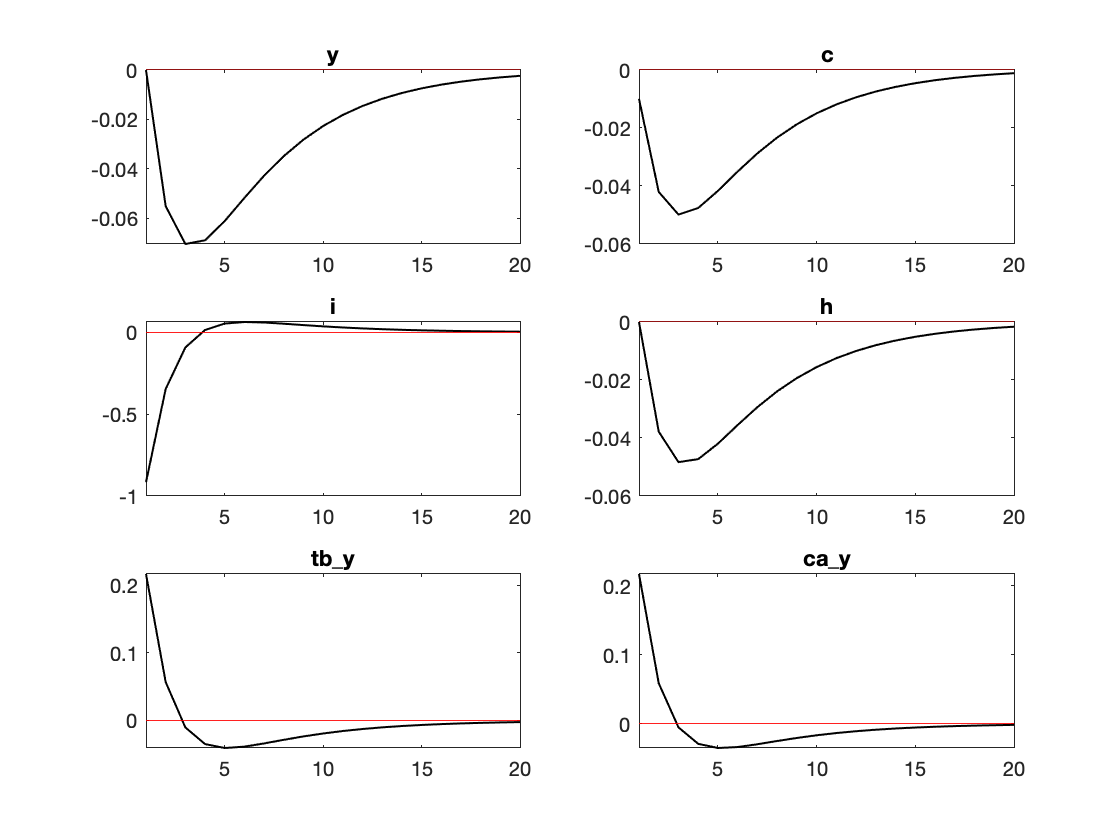
\includegraphics[width=.95\linewidth]{figure_0.png}
\end{center}

Intuition for the IRFs
\begin{itemize}
  \item A rise in interest rate makes borrowing more costly (note that the steady state debt level is positive), thus the economy consumes less and saves more to pay back the debt. Thus, $c$ drops but $\frac{tb}{y}$ and $\frac{ca}{y}$ increase.
  \item Investment further drops because of the high interest rate.
  \item Due to GHH utility, there is no wealth effect in labor supply. Because $i \downarrow \to K \downarrow \to MPL = w \downarrow$, employment $h$ also drops. Meanwhile, $y$ drops.
\end{itemize}




\subsection*{Q2. The IDF Model}

\begin{matlabcode}
% replicate column 1 of table 4.4
% make sure the results generated by the new model is consistent with the old results

dynare IDF
\end{matlabcode}
\begin{matlaboutput}
THEORETICAL MOMENTS
VARIABLE         MEAN  STD. DEV.   VARIANCE
y              0.3964     0.0307     0.0009
c              0.1106     0.0235     0.0006
i             -1.0795     0.0910     0.0083
h              0.0074     0.0211     0.0004
tb_y           0.0200     0.0155     0.0002
ca_y           0.0000     0.0146     0.0002

MATRIX OF CORRELATIONS
Variables         y       c       i       h    tb_y    ca_y
y            1.0000  0.9376  0.6581  1.0000 -0.0122  0.0263
c            0.9376  1.0000  0.5581  0.9376 -0.0701  0.0623
i            0.6581  0.5581  1.0000  0.6581 -0.7025 -0.7301
h            1.0000  0.9376  0.6581  1.0000 -0.0122  0.0263
tb_y        -0.0122 -0.0701 -0.7025 -0.0122  1.0000  0.9609
ca_y         0.0263  0.0623 -0.7301  0.0263  0.9609  1.0000

COEFFICIENTS OF AUTOCORRELATION
Order          1       2       3       4       5
y         0.6122  0.3505  0.1925  0.1029  0.0539
c         0.6988  0.4959  0.3725  0.3010  0.2604
i         0.0700 -0.1405 -0.1415 -0.0995 -0.0612
h         0.6122  0.3505  0.1925  0.1029  0.0539
tb_y      0.3268  0.1113  0.0531  0.0440  0.0473
ca_y      0.3022  0.0657 -0.0061 -0.0228 -0.0232
Total computing time : 0h00m01s
Note: warning(s) encountered in MATLAB/Octave code
\end{matlaboutput}

We can see that the moments reported in Dynare are basically the same as in table 4.4.

Now we turn off the TFP shock and turn on the interest rate shock.

\begin{matlabcode}

% turn off productivity shock and turn on interest rate shock
set_param_value('sigma_tfp', 0);
set_param_value('sigma_mu',  0.012);

% re-run the model
options_.irf = 20; 
[info,oo_,options_,M_]=stoch_simul(M_,options_,oo_,var_list_);
\end{matlabcode}
\begin{matlaboutput}
THEORETICAL MOMENTS
VARIABLE         MEAN  STD. DEV.   VARIANCE
y              0.3964     0.1622     0.0263
c              0.1106     0.1162     0.0135
i             -1.0795     1.0224     1.0454
h              0.0074     0.1115     0.0124
tb_y           0.0200     0.2513     0.0632
ca_y           0.0000     0.2470     0.0610

MATRIX OF CORRELATIONS
Variables         y       c       i       h    tb_y    ca_y
y            1.0000  0.9884  0.0684  1.0000  0.2254  0.1724
c            0.9884  1.0000  0.2005  0.9884  0.0912  0.0388
i            0.0684  0.2005  1.0000  0.0684 -0.9562 -0.9709
h            1.0000  0.9884  0.0684  1.0000  0.2254  0.1724
tb_y         0.2254  0.0912 -0.9562  0.2254  1.0000  0.9983
ca_y         0.1724  0.0388 -0.9709  0.1724  0.9983  1.0000

COEFFICIENTS OF AUTOCORRELATION
Order          1       2       3       4       5
y         0.9259  0.8018  0.6712  0.5513  0.4481
c         0.9436  0.8205  0.6843  0.5570  0.4464
i         0.3781  0.0976 -0.0214 -0.0654 -0.0758
h         0.9259  0.8018  0.6712  0.5513  0.4481
tb_y      0.3422  0.0515 -0.0666 -0.1056 -0.1099
ca_y      0.3282  0.0438 -0.0712 -0.1086 -0.1119
\end{matlaboutput}

The impulse response functions are shown as follows:
\begin{center}
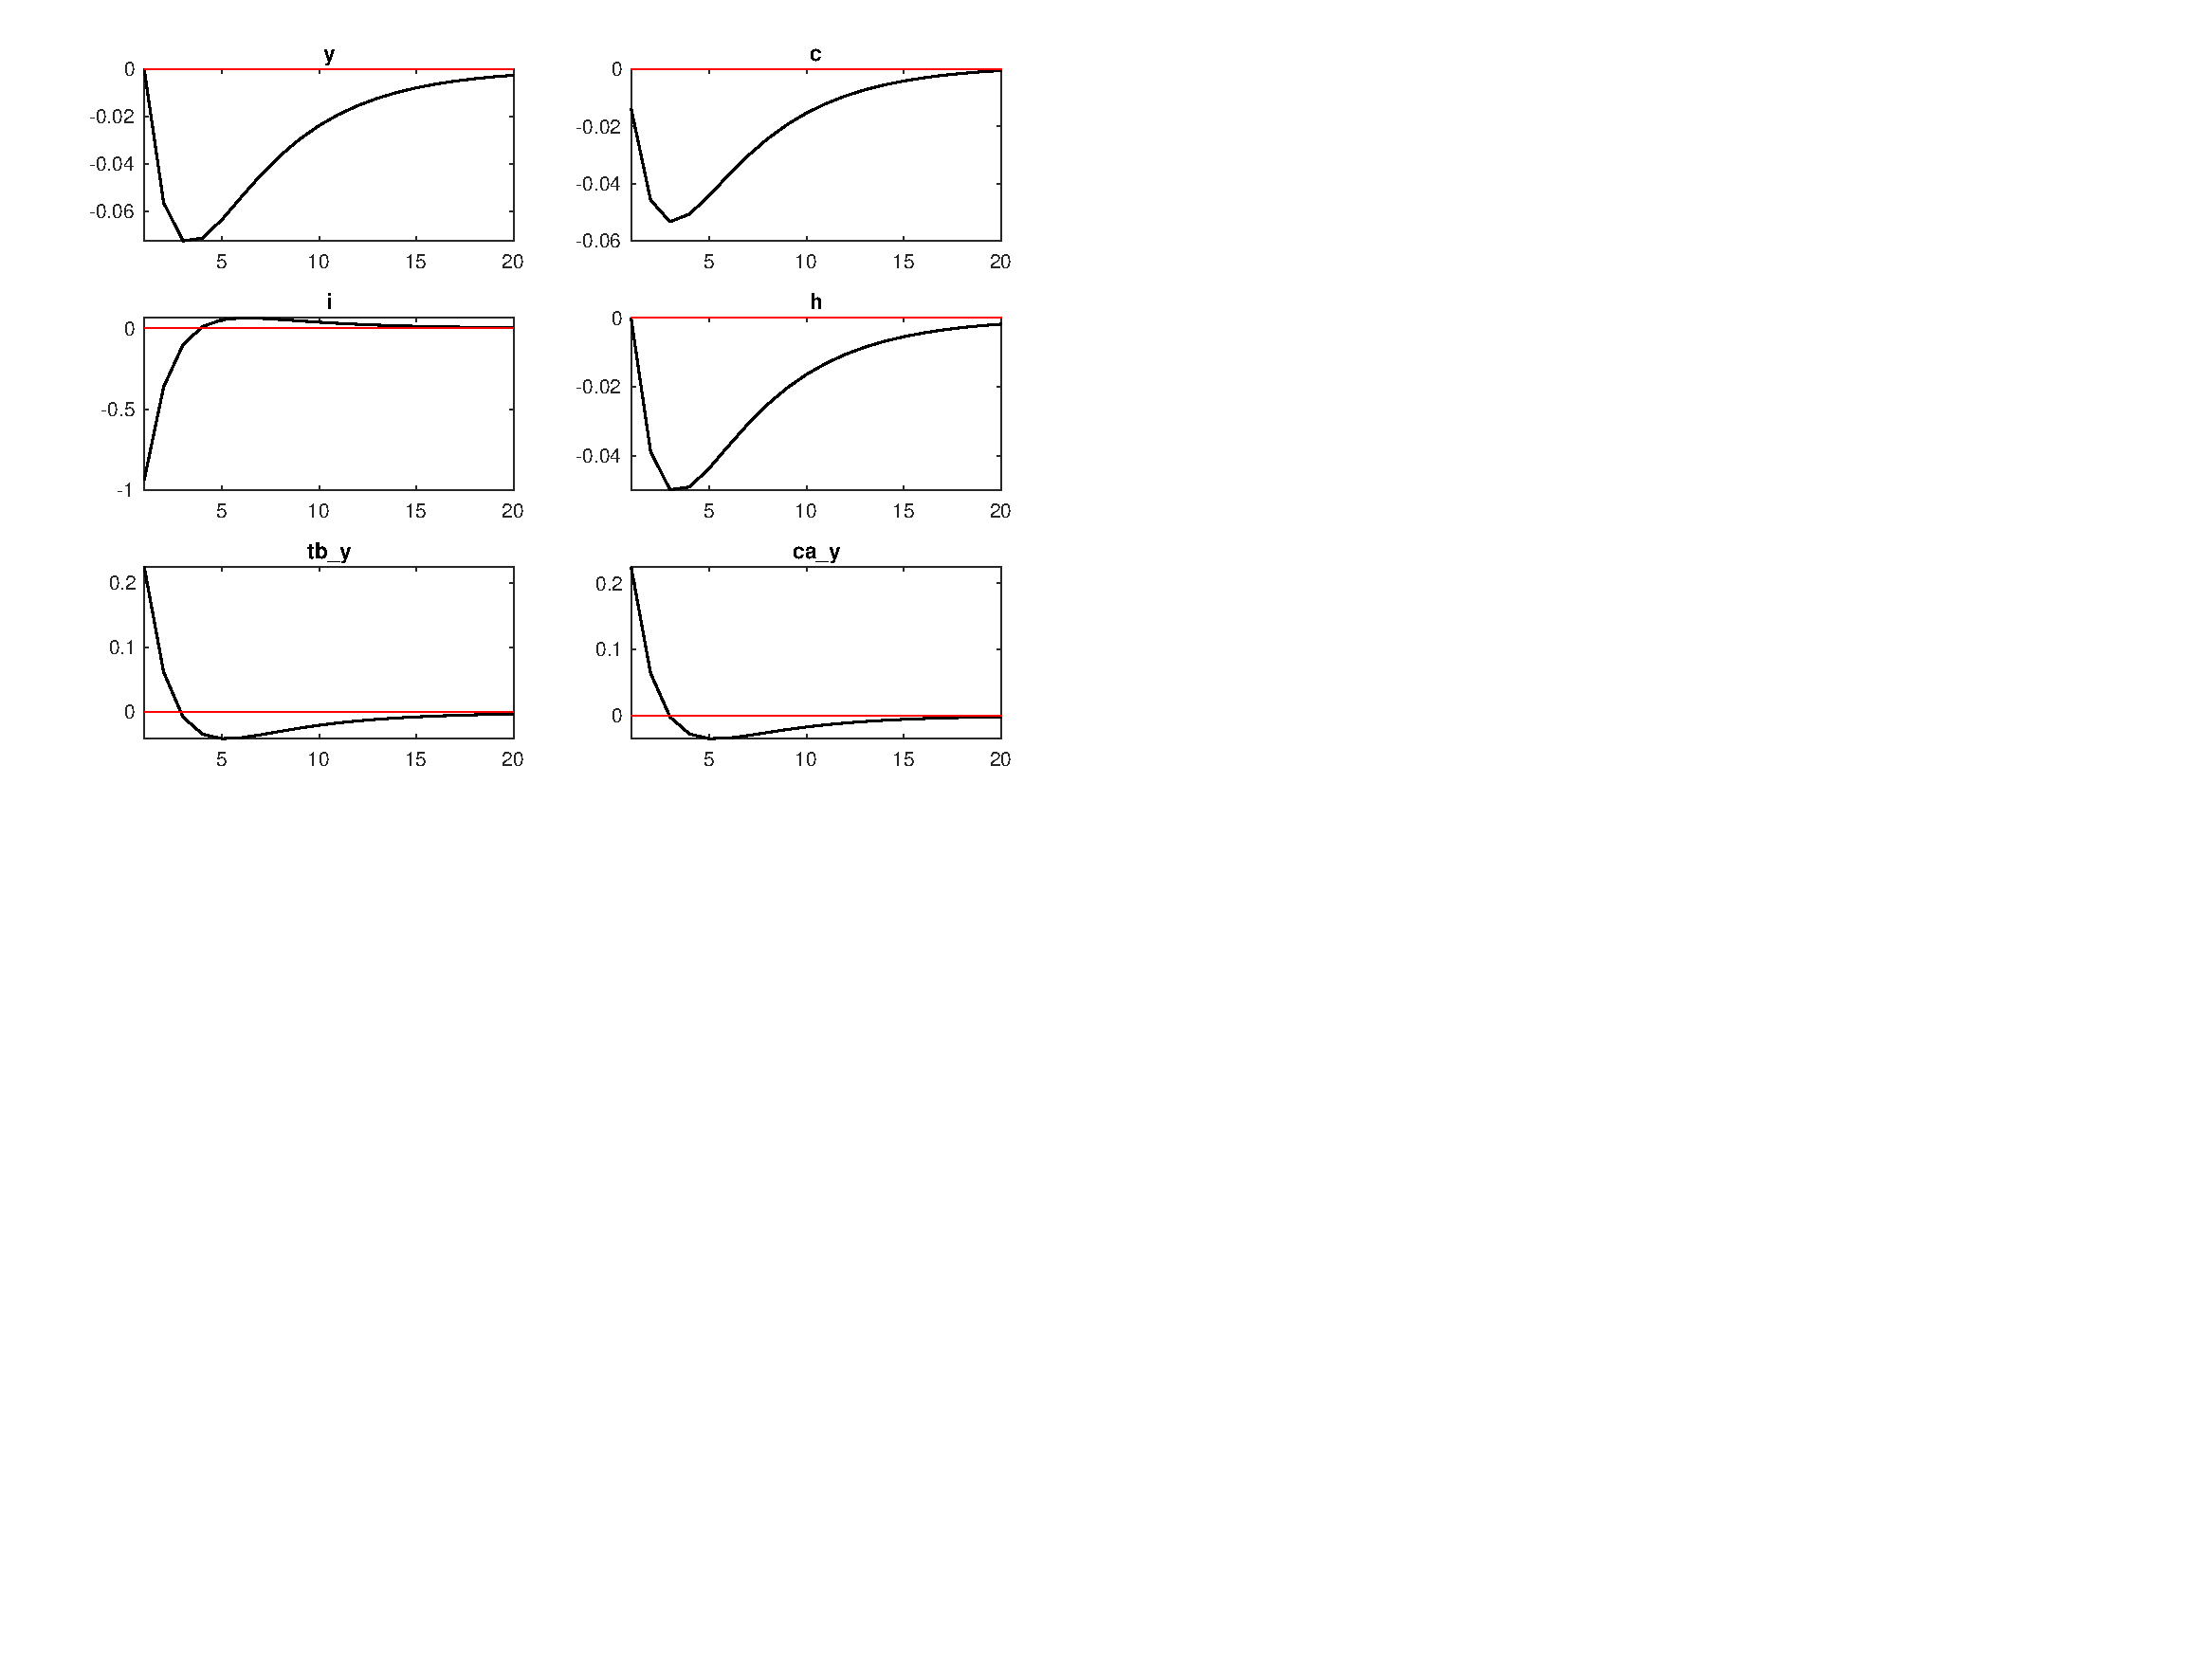
\includegraphics[width=.95\linewidth]{figure_1.pdf}
\end{center}

These IRFs are very similar to the ones in Q1. The intuitions are the same as in Q1.

\subsection*{Q3. Comparisons}

In terms of IRFs, the two models generate almost exactly the same IRFs. As for statistic moments, we summarize earlier findings in a table below. The results are very similar.

\begin{table}[hb]
    \centering
    \begin{tabular}{lrrrr}
    \hline
                            & IDF & EDEIR \\ \hline
    \textbf{Volatilities}\\
    std$(y)$                & 16.2 & 15.6       \\ 
    std$(c)$                & 11.6 & 10.9       \\ 
    std$(i)$                &102.2 & 99.3       \\ 
    std$(h)$                & 11.2 & 10.7       \\ 
    std$(\frac{tb}{y})$     & 25.1 & 24.2       \\ 
    std$(\frac{ca}{y})$     & 24.7 & 23.8       \\ 
    \textbf{Serial Correlations}\\
    corr$(y_{t},y_{t-1})$   & 0.93 & 0.92       \\ 
    corr$(c_{t},c_{t-1})$   & 0.94 & 0.94       \\ 
    corr$(i_{t},i_{t-1})$   & 0.38 & 0.37       \\ 
    corr$(h_{t},h_{t-1})$   & 0.93 & 0.92       \\ 
    corr$(\frac{tb_t}{y_t},\frac{tb_{t-1}}{y_{t-1}})$  & 0.34 & 0.33 \\ 
    corr$(\frac{ca_t}{y_t},\frac{ca_{t-1}}{y_{t-1}})$  & 0.33 & 0.32 \\ 
    \textbf{Correlations with Output}\\
    corr$(c_{t},y_{t})$     & 0.99 & 0.99       \\ 
    corr$(i_{t},y_{t})$     & 0.07 & 0.06       \\ 
    corr$(h_{t},y_{t})$     & 1.00 & 1.00       \\ 
    corr$(\frac{tb_t}{y_t}, y_{t})$  & 0.23 & 0.24       \\ 
    corr$(\frac{ca_t}{y_t}, y_{t})$  & 0.17 & 0.19       \\ \hline
    \end{tabular}
\end{table}

\end{document}
